\section{Sensing Methods}
\label{sec:sensing}
This section covers sensing methods for recording signals which are informative of lubrication conditions in ball bearings. The section presents a taxonomy for categorising sensing methods and presents the methods grouped accroding to this taxonomy.

\subsection{Sensing Methods Taxonomy}
We classify sensing methods for online LCM of ball bearings along two independent axes. A method is \textbf{active} if it supplies external energy into the bearing system to probe its response; it is \textbf{passive} if it relies solely on signals generated by the bearing under operation. A method is \textbf{invasive} if it requires unobstructed access to the lubricant film, direct physical contact with the lubricant, sensors mounted inside the bearing, or structural modifications to the bearing or its housing; it is \textbf{non-invasive} if none of these requirements apply. Online and in-line monitoring modes are defined in Section~\ref{sec:intro}.

These two axes define four categories illustrated in Figure~\ref{fig:taxonomy}: active/invasive, active/non-invasive, passive/invasive, and passive/non-invasive. Notice that passive/invasive methods is empty: the methods eligible for this category did not qualify as online or in-line, e.g. oil sampling.

In general, the current active methods directly measure the relevant quantities, e.g. lubricant contamination or film thickness, while passive methods rely on signals which arise as a consequence of changing lubrication conditions. The passive methods are therefore more indirect and function as proxy measures for lubrication conditions. The passive/non-invasive category is, nevertheless, of particular industrial relevance because its methods can be applied to bearings in service without modification and without interrupting operation. The present review covers all four categories for completeness but gives greatest depth to the passive/non-invasive methods given their greater industrial applications and more significant current research gap.

\begin{figure}[H]
\centering
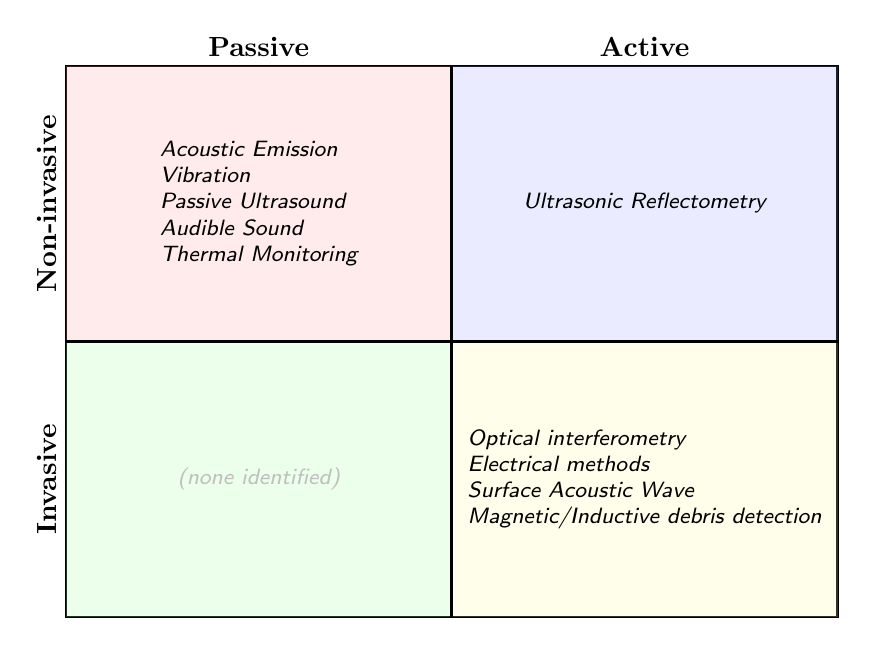
\begin{tikzpicture}
    % ===== PARAMETERS =====
    \pgfmathsetmacro{\W}{7}    % total width
    \pgfmathsetmacro{\H}{5}    % total height
    \pgfmathsetmacro{\S}{1.4}  % global scale factor
    \pgfmathsetmacro{\LW}{1}   % line width in pt

    % Derived midpoints
    \pgfmathsetmacro{\Mx}{\W/2}
    \pgfmathsetmacro{\My}{\H/2}

    \begin{scope}[scale=\S]

        % ===== DRAWING =====
        % Outer rectangle
        \draw[line width=\LW pt] (0,0) rectangle (\W,\H);

        % Softer, semi-transparent colors
        \fill[red!40,    opacity=0.2] (0,\My) rectangle (\Mx,\H);
        \fill[blue!40,   opacity=0.2] (\Mx,\My) rectangle (\W,\H);
        \fill[green!40,  opacity=0.2] (0,0) rectangle (\Mx,\My);
        \fill[yellow!40, opacity=0.2] (\Mx,0) rectangle (\W,\My);

        % Dividing lines
        \draw[line width=\LW pt] (0,\My) -- (\W,\My);
        \draw[line width=\LW pt] (\Mx,0) -- (\Mx,\H);

        % ===== TEXT OUTSIDE BOXES =====
        % Top labels (centered above top squares)
        \node[anchor=south] at (\Mx/2, \H) {\textbf{Passive}};
        \node[anchor=south] at (\Mx + \Mx/2, \H) {\textbf{Active}};

        % Left labels (vertical, centered beside left squares)
        \node[anchor=south, rotate=90] at (0, \My + \My/2) {\textbf{Non-invasive}};
        \node[anchor=south, rotate=90] at (0, \My/2) {\textbf{Invasive}};

        % ===== TEXT INSIDE BOXES =====
        % ===== TEXT STYLE =====
        \tikzset{
            boxtext/.style={
                font=\sffamily\itshape\footnotesize,
                text=black                     % text color
            }
        }
        % Centers of each quadrant
        \node[boxtext] at (\Mx/2,        \My + \My/2) {
            \begin{tabular}{l}
                Acoustic Emission \\
                Vibration \\
                Passive Ultrasound \\
                Audible Sound \\
                Thermal Monitoring
            \end{tabular}
        };
        \node[boxtext] at (\Mx + \Mx/2,  \My + \My/2) {
            \begin{tabular}{l}
                Ultrasonic Reflectometry\\
            \end{tabular}
        };
        % Passive/Invasive quadrant intentionally left empty — see caption
        \node[boxtext, text=gray!50, font=\sffamily\itshape\footnotesize] at (\Mx/2, \My/2) {(none identified)};
        \node[boxtext] at (\Mx + \Mx/2,  \My/2)       {
            \begin{tabular}{l}
                Optical interferometry \\
                Electrical methods \\
                Surface Acoustic Wave \\
                Magnetic/Inductive debris detection \\
            \end{tabular}
        };

    \end{scope}
\end{tikzpicture}
\caption{Classification of sensing methods for lubrication condition monitoring along two independent axes: active vs.\ passive signal acquisition, and invasive vs.\ non-invasive installation requirements. The passive/invasive quadrant contains no identified methods: sensing methods that require physical access to the lubricant (invasive) almost invariably do so to supply or measure a controlled excitation (active).}
\label{fig:taxonomy}
\end{figure}

\noindent The subsections below describe each sensing modality with a standardised structure: (i) physical principle, (ii) what lubrication information it is sensitive to, (iii) sensor hardware and technology considerations, and (iv) installation and operational characteristics. Signal processing methods are treated in depth in Section~\ref{sec:sp}. A factor common to all modalities is the transmission path between the signal origin and the sensor, which is treated first as it governs which signals are accessible at the sensor regardless of modality.

% ─────────────────────────────────────────────────────────────────────────────
\subsection{Signal Transmission Path and Attenuation}
\label{subsec:transmission}

All online sensing methods for LCM share a fundamental constraint: the sensor cannot be placed at the signal origin. The bearing contact zone -- where asperity contacts, lubricant film formation, and wear events occur -- is physically inaccessible to a sensor. Any measurable signal must first propagate from the contact zone to the sensor through a series of solid media and mechanical interfaces. Understanding this transmission path is not merely a practical installation concern It directly constrains which signal processing operations are valid, which frequency bands are informative, and how results from laboratory rigs transfer to industrial deployments.

For a sensor mounted on the bearing housing, the signal originates at the ball--raceway contact zone on the outer ring and propagates through two sequential material bodies and their connecting interfaces: bulk propagation through the outer ring, the outer ring--housing bore interface (press fit, clearance fit, or clamped, depending on the bearing arrangement), bulk propagation through the housing, and the sensor coupling layer. Each interface boundary introduces frequency-dependent attenuation; cumulative losses over a typical path through the outer ring and the ring--housing interface mean that a 500\,kHz AE signal may arrive at the sensor attenuated by 30--60\,dB relative to the source \cite{ono_comprehensive_2020,scheeren_evaluation_2022}. This range spans the difference between a detectable signal and pure noise. For active methods such as ultrasonic reflectometry and SAW sensing, the path is traversed twice, compounding the problem. The transmission path therefore acts as a low-pass filter whose effect increases with the number of transmission interfaces and the length of the transmission path. This path is illustrated in Figure~\ref{fig:transmission_path}.

\begin{figure}[H]
\centering
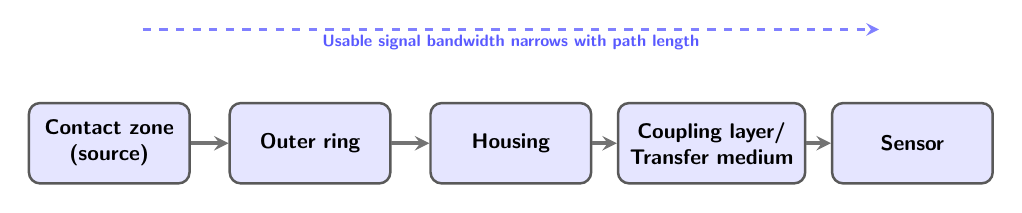
\begin{tikzpicture}[
  scale=0.85, transform shape,
  blk/.style={rectangle, rounded corners=4pt, draw=black!65, line width=0.9pt,
              fill=blue!10, minimum width=2.4cm, minimum height=1.2cm,
              align=center, font=\sffamily\small\bfseries, inner sep=5pt},
  arr/.style={->, >=stealth, line width=1.3pt, black!55},
  darr/.style={->, >=stealth, line width=1.0pt, dashed, blue!50},
]

% Blocks
% Contact zone lies on the outer ring's own raceway surface (not a separate
% body), so the arrow into it is bulk propagation within the ring, not a
% material interface. The outer ring--housing joint is left as a plain arrow
% (no label): its exact nature -- press fit, clearance fit, clamped, etc. --
% is application-specific, so it is not asserted here. The sensor coupling
% layer is a genuine distinct material regardless of mounting style, so it
% gets its own block rather than an arrow label.
\node[blk]  (SRC) at (0,0)     {Contact zone\\(source)};
\node[blk]  (OR)  at (3.0,0)   {Outer ring};
\node[blk]  (HSG) at (6.0,0)   {Housing};
\node[blk]  (CPL) at (9.0,0)   {Coupling layer/ \\ Transfer medium};
\node[blk]  (SEN) at (12.0,0)  {Sensor};

% Arrows between blocks (unlabelled -- see note above)
\draw[arr] (SRC.east) -- (OR.west);
\draw[arr] (OR.east)  -- (HSG.west);
\draw[arr] (HSG.east) -- (CPL.west);
\draw[arr] (CPL.east) -- (SEN.west);

% Bandwidth arrow (top, spanning full path)
\node[font=\sffamily\scriptsize\bfseries, text=blue!65] at (6.0, 1.5)
  {Usable signal bandwidth narrows with path length};
\draw[darr] (0.5,1.7) -- (11.5,1.7);

\end{tikzpicture}
\caption{Signal transmission path from the ball--raceway contact zone to a housing-mounted sensor. The interface between the outer ring and housing bore -- press fit, clearance fit, or clamped, depending on the bearing arrangement -- is the dominant attenuation element for high-frequency content. Cumulative path losses of 30--60\,dB at 500\,kHz render the usable frequency bandwidth at the sensor geometry-, mounting-, and material-specific, limiting the transferability of signal processing configurations across experimental setups.}
\label{fig:transmission_path}
\end{figure}

This has two direct consequences for signal processing.

First, frequency-domain configurations derived from one experimental setup do not automatically transfer to another. The frequency content including the resonant frequencies of the housing structure and the spectral bandwidth and intensity of the content observable at the sensor are all geometry-specific. This limits the portability of signal processing configurations tuned on laboratory test rigs to industrial deployments with different sensor placements, housing geometries, or coupling conditions.

Second, sensor placement is a signal processing decision, not only an installation practicality. Mounting a sensor across a bolted flange, a material transition, or a long structural path can render high-frequency content undetectable regardless of sensor sensitivity and distort other frequency content in unpredicted ways. For non-contact microphone monitoring, the additional transmission from the housing surface into air is frequency-dependent: audible sound (20\,Hz--20\,kHz) propagates relatively efficiently, but ultrasonic frequencies ($>$40\,kHz) undergo rapid geometric spreading and air absorption \cite{carotenuto_ranging_2021}, limiting non-contact acoustic monitoring to the audible and near-ultrasonic range.

% ─────────────────────────────────────────────────────────────────────────────
\subsection{Passive and Non-Invasive Methods}
\label{subsec:passive_noninv}

\subsubsection{Acoustic Emission}
\label{subsubsec:ae}

\paragraph{Physical principle.} Acoustic emission (AE) refers to transient, high-frequency elastic stress waves -- typically in the range 20\,kHz to 1\,MHz -- spontaneously generated within the bearing material and contact interfaces as a result of tribological processes. These processes include asperity contact and micro-fracture under inadequate lubrication, crack initiation and propagation under contact stress, wear particle generation, and frictional energy release at rolling and sliding contacts \cite{hou_-situ_2025,delft_university_of_technology_tu_delft_influence_2024,scheeren_acoustic_2024}.

\paragraph{Literature on LCM.} AE is sensitive to the lubrication regime: as the specific film thickness $\Lambda$ decreases from EHL toward boundary lubrication, asperity contacts increase in frequency and severity, generating more AE energy.

% Energy/amplitude
This is demonstrated by multiple sources: Cornel et al.\ \cite{cornel_condition_2021} find an inverse correlation between AE amplitude and $\Lambda$ in cylindrical roller bearings under controlled lubrication conditions; Hou and Zhang \cite{hou_-situ_2025} show that amplitude and energy features from AE signals in thrust ball bearings map onto distinct lubrication regime clusters and can be used to estimate $\Lambda$ with high accuracy;  Miettinen et al.\ \cite{miettinen_analysis_2001} show that the pulse count rate increases monotonically with grease starvation. An important exception to the monotonic amplitude-lubrication relationship is the non-monotonic energy response observed by Hou and Zhang, in which transitioning from dry contact to low-viscosity lubrication initially \textit{decreases} AE energy before it rises again with increasing viscosity due to viscous damping forces on the bearing ring. This highlights that AE-lubrication relationships are configuration-specific and require calibration.

Zhang et al.\ \cite{zhang_coupled_2026} provide a mechanistic account of lubricant-dependence: in cylindrical roller bearing tests with greases of distinct viscosities, they show AE arises from two different sources: asperity contact (RMS scaling with the square root of speed) and lubricant friction (RMS scaling quadratically with speed). They furthermore show that high-viscosity grease produces friction-dominated AE signals which are strongly speed-dependent, while AE signals from low-viscosity grease are more asperity-contact dominated. They additionally show that low-viscosity grease produces more strongly fluctuating AE than high-viscosity grease across all frequency sub-bands.

Tandon et al.\ \cite{tandon_condition_2007} compare vibration, AE, stator current, and shock pulse for grease contamination detection in electric motor ball bearings, finding AE most effective for early-stage contamination detection.

\paragraph{Sensor technology.}
% TODO: this paragraph's hardware claims are largely uncited. Need a citation for: "almost exclusively piezoelectric" / resonant vs. wideband sensor taxonomy; the 100kHz--1MHz wideband flat-response range; and the >500kHz sampling-rate requirement. The ADI "Predictive Maintenance Sensor Performance Specifications" article (\cite{murphy_choosing_2020}, added for the Vibration/Sound sections) does not cover AE sensors, so a dedicated AE-hardware reference (datasheet, standard, or review) is needed here.
AE sensors are almost exclusively piezoelectric, available in two configurations with different SNR--bandwidth trade-offs. Resonant sensors are tuned to a single resonant frequency providing very high sensitivity in a narrow bandwidth but discarding spectral content outside that band. Wideband sensors sacrifice sensitivity for a nominally flat response across 100\,kHz to 1\,MHz, which are more suited for the frequency-domain and time-frequency signal processing methods reviewed in Section~\ref{sec:sp}. For LCM applications where the informative frequency content is a priori unknown or lubrication-condition-dependent, wideband sensors are preferable. Sensor-to-housing coupling (adhesive bond, magnetic mounting, or grease couplant) is a significant source of variability: a poorly bonded sensor can introduce 10--20\,dB of additional loss at high frequencies \cite{scheeren_evaluation_2022}, making coupling consistency a prerequisite for any quantitative AE feature.

Since AE signals are high frequency, they require a high sample rate (>500\,kHz) to adequately capture all content. This poses a challenge since large data volumes are generated by continuous AE acquisition at the required sampling rates, which most studies address through windowed statistical features, interval sampling, or event-triggered recording.

\subsubsection{Vibration}
\label{subsubsec:vibration}

\paragraph{Physical principle.} Vibration signals are sensitive to lubrication conditions through two mechanisms: (1) impulsive excitation from asperity contacts at inadequate $\Lambda$, increasing broadband vibration energy, and (2) changes in the rolling element bearing dynamics (stiffness, damping) associated with changes in the lubrication film.

\paragraph{Literature on LCM.} Vibration-based condition monitoring is the most mature and industrially widespread sensing approach for rolling element bearings, with a substantial body of literature on bearing fault detection and remaining useful life estimation \cite{randall_vibrationbased_2021,rai_review_2016}. Its application to lubrication condition monitoring is more limited, primarily because lubrication-related processes excite frequency content above 30\,kHz, which lies at or beyond the upper limit of typical accelerometers and requires dedicated high-frequency accelerometers or acoustic emission sensors \cite{jakobsen_detecting_2023}. Jakobsen et al.\ \cite{jakobsen_vibration_2021} demonstrate that vibration statistics and spectral kurtosis are correlated with $\kappa$ values and can be used to predict lubrication adequacy. Xu et al.\ \cite{xu_vibration-based_2024} show that minimum entropy deconvolution applied to vibration signals enhances weak impulsive events associated with lubricant starvation, improving detectability. Zhang et al.\ \cite{zhang_interpretable_2026} target grease-lubricated bearings specifically, classifying lubrication state into insufficiency, degradation, and contamination from vibration using a deep-learning pipeline rather than handcrafted statistics.

\paragraph{Sensor technology.}
% TODO: this paragraph's accelerometer bandwidth figures now follow \cite{murphy_choosing_2020} (Table 3: MEMS accelerometer, DC-capable, 3--20\,kHz+ -3dB bandwidth across available devices; piezoelectric accelerometer, no DC response, 2.5--30\,kHz+ -3dB bandwidth across available devices). Two other places in the paper still state the older DC--1--5/7--10/15--50kHz tiered breakdown and need to be brought in line with this: Table~\ref{tab:signal_origins} row 2 (physical_origins_of_signals.tex) and the "$\leq$50\,kHz" vibration sampling-rate figure in Table~\ref{tab:deployment} (comparative_analysis.tex).
Two accelerometer technologies are relevant to LCM, with fundamentally different characteristics. MEMS accelerometers respond from 3\,kHz up to more than 20\,kHz but not significantly above 30khz, missing a large part of the informative band for LCM, which lies above 30\,kHz. Piezoelectric accelerometers offer wider bandwidths, from 2.5\,kHz up to more than 30\,kHz across available devices \cite{murphy_choosing_2020}. The highest-bandwidth piezoelectric parts therefore reach into part of the LCM-informative range but typically at reduced sensitivity relative to their lower-bandwidth counterparts. The consistent finding in the reviewed literature that vibration-based LCM is limited compared to AE and passive ultrasound reflects this hardware constraint: the most LCM-relevant signal content lies at or beyond the practical range of standard industrial accelerometers \cite{jakobsen_detecting_2023}.

\subsubsection{Ultrasound}
\label{subsubsec:ultrasound_passive}

\paragraph{Physical principle.} Ultrasound signals are generated passively by the bearing itself and require no external excitation. These signals are generated by friction, wear, and asperity contacts in the bearing and therefore contain information on lubrication state and changes. Ultrasound signals as such respond to these changes earlier in the degradation process than lower-frequency vibration \cite{jakobsen_detecting_2023}.

\paragraph{Literature on LCM.} Passive ultrasound monitoring is currently used industrially for LCM. Products such as UE Systems Ultraprobe \cite{ue_systems_ultraprobe_2026}, Sonotec, and AccuTrak employ threshold-based methods that compare the measured ultrasound level against a baseline established under adequate lubrication conditions, instructing relubrication when the level rises a specified number of dB above the reference \cite{lineham_ultrasonic_2008}. Jakobsen et al.\ \cite{jakobsen_detecting_2023} demonstrate that more sophisticated processing of passive ultrasound -- using band-pass filtering, time-domain features, and regression models -- can predict $\kappa$ values rather than just threshold exceedances.

\paragraph{Sensor technology.}
% TODO: ADI "Predictive Maintenance Sensor Performance Specifications" (Table 3), now cited as \cite{murphy_choosing_2020}, lists MEMS ultrasonic microphone bandwidth as ~100kHz and MEMS microphone (non-ultrasonic) as ~20kHz. The 20kHz figure is now cited on the Audible Sound MEMS-microphone claim below; the 100kHz figure could replace "have not yet been systematically evaluated" with a concrete bandwidth citation (murphy_choosing_2020) for MEMS ultrasonic transducers here, complementing the SPH0641LU (80kHz) example already cited above.
Ultrasonic sensors typically use piezoelectric elements, but their frequency coverage differs by product class. Fixed-threshold sensors often use a narrow resonant band around 35\,kHz to 42\,kHz \cite{ue_systems_ultra-trak_2026,skf_ultrasound_2026}. Some handheld inspection instruments instead offer a much wider, tunable range, e.g.\ 20\,kHz to 100\,kHz in 1\,kHz increments \cite{ue_systems_ultraprobe_2026}. This allows the operator to select a frequency band suited to the fault type being investigated. Garvey \cite{garvey_monitoring_2019} employs a 30\,kHz band of ultrasonic measurements to isolate friction and lubrication related information from mechanical faults. Industrial instruments often translate measurements of ultrasonic signals into the hearable domain to allow human inspection of the sound level and characteristics \cite{lineham_ultrasonic_2008}. In research, low-cost MEMS ultrasonic microphones (e.g.\ SPH0641LU, bandwidth to 80\,kHz) have been demonstrated as an accessible sensor for passive ultrasound LCM \cite{jakobsen_low_2024}. This is still an emerging technology that may enable low-cost, integrated monitoring nodes but their sensitivity and bandwidth characteristics for LCM applications have not yet been systematically evaluated in the reviewed literature.

\subsubsection{Audible Sound (20\,Hz--20\,kHz)}
\label{subsubsec:sound}

\paragraph{Physical principle.} Asperity contacts, friction, and wear events generate broadband mechanical noise, a portion of which is radiated as airborne sound through the bearing housing. Changes in lubrication regime alter the amplitude and spectral distribution of this emission. Georgiev et al.\ \cite{georgiev_microphone_2017} demonstrate that frequency-domain features extracted from microphone array measurements show measurable changes as lubrication levels vary, and propose classification via fuzzy logic or neural networks.

\paragraph{Sensor technology.}
% TODO: the 30dB(A) SPL noise-floor figure below is still uncited. Do not cite murphy_choosing_2020 for it -- that source reports MEMS microphone noise as a 57--74dB SNR figure, a different metric, not an SPL noise floor. Only the 20kHz bandwidth figure is corroborated by murphy_choosing_2020.
The practical advantage of microphone-based monitoring is its fully non-contact nature, enabling installation without any access to the bearing. MEMS microphones now achieve noise floors below 30\,dB(A) with flat frequency response to 20\,kHz \cite{murphy_choosing_2020}, making them suitable for bearing monitoring at very low cost. The main limitation is susceptibility to ambient noise in industrial environments. Signal quality is highly dependent on the acoustic environment of the installation and roximity to the bearing and ambient noise influence the measurements.

\subsubsection{Thermal Monitoring}
\label{subsubsec:thermal}

\paragraph{Physical principle.} Heat generation is caused by friction and wear inside the bearing, serving as an indicator of lubrication regime. Under adequate EHL lubrication, viscous heat generation is modest and as the bearing transitions to mixed or boundary lubrication, frictional heat increases significantly \cite{yan_thermal_2019}.

\paragraph{Literature on LCM.} Moussa et al.\ \cite{moussa_passive_2017} demonstrate a passive thermography approach to bearing condition monitoring in which temperature trend analysis provides early-warning capability. The primary physical limitation of thermal monitoring for LCM is its slow response, since heat must build up and diffuse through the bearing before it is detectable. Temperature rise is therefore a downstream consequence of sustained inadequate lubrication, making the approach better suited to early warning of developing degradation trends than to detection of transient lubrication events.

\paragraph{Sensor technology.}
Thermocouples and resistance temperature detectors provide point measurements with response times of seconds to tens of seconds, which is adequate for trend monitoring but not for transient events. Infrared thermography cameras provide spatially temperature maps without contact but require line-of-sight to the bearing housing surface. Fibre Bragg grating sensors, demonstrated by Janssens et al.\ \cite{janssens_thermal_2015} and Mohammed et al.\ \cite{mohammed_electric_2021}, offer both thermal and mechanical (vibration) sensing in a single fibre.

% ─────────────────────────────────────────────────────────────────────────────
\subsection{Active Methods}
\label{subsec:active}

\subsubsection{Active Ultrasonic Reflectometry}
\label{subsubsec:ultrasonic_active}

\paragraph{Physical principle.} Active ultrasonic methods transmit high-frequency (1--200\,MHz) pulses from a piezoelectric transducer into the bearing raceway. At the interface between the raceway and the lubricant film, a portion of the wave is reflected. The reflection coefficient depends on the acoustic impedance of the lubricant film, which is a function of both film thickness and lubricant bulk modulus. Using physics-based acoustic propagation models -- most commonly the quasi-static spring-layer model \cite{drinkwater_ultrasonic_2009} -- the film thickness can be recovered from the measured reflection coefficient.

\paragraph{Literature on LCM.} Active ultrasonic methods can provide quantitative, real-time measurement of EHL film thickness under operating conditions and has been covered in multiple papers \cite{dwyer-joyce_measurement_2003,zhang_ultrasonic_2015,chen_evaluation_2023,wu_ultrasonic_2025}. Li et al.\ \cite{li_lubrication_2026} extend this to the wind turbine pitch bearing, demonstrating film thickness measurement via ultrasonic reflection in a large-scale industrial component. Chen et al.\ \cite{chen_sub-nyquist_2025} address the data-volume challenge of high-frequency ultrasonic acquisition using sub-Nyquist sampling. The tribo-acoustic tachometer of Tatzgern et al.\ \cite{tatzgern_tribo-acoustic_2025} additionally recovers cage rotational speed from the same ultrasonic reflection signal, providing simultaneous kinematic and lubrication information from a single device.

\paragraph{Sensor technology.} Although transducers can in principle be mounted externally on the bearing housing, the requirement for precise transducer coupling, alignment, and calibration creates practical barriers to deployment on standard industrial bearings that are not present for passive sensing methods \cite{hansen_comparison_2022,wang_accuracy-improved_2024}.

\subsubsection{Electrical Methods}
\label{subsubsec:electrical}

\paragraph{Physical principle.} Electrical sensing methods treat the ball bearing and lubricant as elements of an electrical circuit. An externally applied electrical signal -- voltage or current -- probes the electrical properties of the lubricant film, which change with film thickness, lubricant degradation, and debris content.

\paragraph{Literature on LCM.} Three variants are used and are described extensively in reviews: electrical capacitance \cite{cen_ehl_2021,dai_situ_2024,schneider_method_2022}, electrical impedance \cite{becker-dombrowsky_electrical_2024,maruyama_lubrication_2023}, and electrical resistance \cite{maruyama_lubrication_2019}. All require an externally applied electrical signal, making them active methods. Grease-lubricated bearings present additional modelling challenges due to the heterogeneous dielectric properties of the thickener matrix \cite{cojocaru_grease_2025,zhang_grease_2021}.

\subsubsection{Surface Acoustic Wave Sensing}
\label{subsubsec:saw}
Surface acoustic waves (SAWs) are acoustic waves propagating along the surface of elastic materials with rapid depth decay. Piezoelectric probes actively excite SAWs that travel along the raceway surface. As these waves interact with the lubricant film, energy is transferred to the fluid causing wave attenuation, while the lubricant loading also shifts the wave velocity, producing a measurable time delay at a receiving transducer. Both attenuation and time delay of the induced wave can thus be related to lubrication film thickness and condition \cite{lindner_a23_2011}.

\subsubsection{Optical Methods}
\label{subsubsec:optical}
Optical methods use light-based techniques to either measure lubricant film thickness directly or detect and classify wear debris.

\paragraph{Optical film thickness measurement.}
Optical interferometry and laser-induced fluorescence are the reference methods for EHL film thickness measurement, underpinning much of the fundamental understanding of EHL contact physics \cite{shang_comprehensive_2024}. Both require optical access to the contact zone and are restricted to purpose-built tribological test rigs with transparent windows -- neither has been demonstrated on standard industrial bearings under field conditions. They are consequently not applicable to online LCM in industrial deployment, but can serve as ground-truth measurement methods against which other sensing approaches are calibrated.

\paragraph{Machine-vision debris detection.}
Machine-vision approaches analyse lubricant debris content using image processing on in-line optical sensors in the lubricant flow path. Liu et al.\ \cite{liu_oil_2022} apply multi-target tracking with Kalman filtering for debris counting and size estimation and Wang et al.\ \cite{wang_online_2022} use a background-difference extraction step followed by convolutional neural network classification to distinguish debris from bubbles, achieving 91.8\% accuracy in a large-diameter, high-flow-rate pipe system. These methods operate on particles in the lubricant flow rather than on the contact zone directly, and can be integrated into oil circulation systems. Unlike interferometry, they are compatible with industrial deployment but provide no film thickness information. Their diagnostic value is therefore for contamination and wear monitoring rather than lubrication regime assessment.

\subsubsection{Magnetic and Inductive Methods}
\label{subsubsec:magnetic}

Magnetic and inductive methods detect metallic wear debris in the lubricant by monitoring perturbations in a magnetic field \cite{sun_online_2021}. An excitation coil generates an alternating magnetic field in or around the lubricant flow path. Ferromagnetic particles perturb the magnetic field primarily through their high permeability, while non-ferrous conductive particles can induce eddy currents that alter the coil impedance. These effects may produce differences in amplitude and phase in the measured signal. Magnetic methods require access to the lubricant flow and are therefore applicable only to oil-circulating systems , meaning that they cannot be used with grease-lubricated or sealed bearings. Shi et al.\ \cite{shi_ultrasensitive_2022} demonstrate an ultrasensitive impedance-based microsensor for oil condition monitoring applicable to small particle sizes.